\documentclass[aip,jcp,reprint,a4paper,onecolumn,nofootinbib,amsmath,amssymb]{revtex4-1}
% Options for onecolumn and a4paper
\linespread{1.0}
\usepackage[expansion,protrusion,tracking=smallcaps]{microtype}
\usepackage{chemformula,tikz}
\usepackage{listings,xcolor}
\lstset{
  basicstyle = \small\ttfamily,
  keywordstyle = \color{blue!80!black},
  commentstyle = \color{green!40!black},
  columns = fullflexible,
  xleftmargin = 1em
}
\lstdefinelanguage{espresso}[]{TCL}{%
  morekeywords={part,reaction,minimize_energy},
  deletekeywords={range}
}
\lstnewenvironment{espresso}[1][]%
  {\lstset{language=espresso,#1}}%
  {}
\lstnewenvironment{bash}[1][]%
  {\lstset{keywordstyle = \color{red!80!blue},keywords={\$},#1}}%
  {}
\usepackage{xspace}
\newcommand\code{\lstinline}
\newcommand{\es}{\mbox{\textsf{ESPResSo}}\xspace}
\newcommand\codees{\lstinline[language=espresso]}
\renewcommand\thefootnote{\fnsymbol{footnote}}
\begin{document}
\title{Catalytic Reactions Tutorial}
\author{Henri Menke}
\email[]{\texttt{henri@icp.uni-stuttgart.de}}
\affiliation{Institute for Computational Physics,
  Universit\"at Stuttgart,
  Allmandring 3,
  D-70569 Stuttgart,
  Germany}
\author{Joost de Graaf}
\email[]{\texttt{jgraaf@icp.uni-stuttgart.de}}
\affiliation{Institute for Computational Physics,
  Universit\"at Stuttgart,
  Allmandring 3,
  D-70569 Stuttgart,
  Germany}
\affiliation{School of Physics and Astronomy,
  University of Edinburgh,
  Scotland, Edinburgh EH9 3JL,
  United Kingdom}
\date{\today}

\begin{abstract}
  In this tutorial we explore how to simulate catalytic reactions using \es\ for the purpose of modeling self-propelled particles (swimmers). We use the implemented scheme to study the enhanced translational diffusion of a catalytic swimmer. This should give a basic idea of how to setup simulations involving a specific type of catalytic reaction in \es\ and enable you to conduct your own numerical experiments with catalytic swimmers.
\end{abstract}

\maketitle

\section{Cataltic Reactions}

Many chemical processes in nature do not occur at room temperature, because the energy penalty is too high for thermal fluctuations to overcome. The activation energy of such processes can in some cases be lowered significantly in the presence of a catalyzer (a catalytic substance). Alternatively, a catalyzer can give access to reaction pathways that are atypical. Below, we discuss this concept in some detail, in order to prepare you for its application to catalytic swimmers.

We may write a general equilibrium reaction as
\begin{equation}
  \label{eq:equi}
  \ch{!(reactants)(R) <=> !(products)(P)}
\end{equation}
where \ch{R} are the reactants and \ch{P} are the products. We restrict ourselves to the situation where there is a single product and single reactant in the following. The double headed arrow is used to indicate that there is a simultaneous forward and backward reaction, which lead to an equilibrium composition of the system. The process in Eq.~\eqref{eq:equi} can be described by the equilbrium reaction constant
\begin{equation}
  \label{eq:const}
  K_{\text{eq}} = \frac{k_{\text{eq},+}}{k_{\text{eq},-}} = \frac{[\ch{P}]}{[\ch{R}]} ,
\end{equation}
with $[\ch{P}]$ and $[\ch{R}]$ the product and reactant concentration and $k_{\textrm{eq},\pm}$ the forward and backward reaction rates, respectively. The primary effect of the reaction is a change of the concentrations of reactants and products over time, whenever the system is brought out of equilibrium, for instance, by adding a large amount of one of the species involved. In that case, the reactions push the system back towards equilibrium,~\textit{i.e.}, a state where they maintain a constant concentration ratio between the products and reactants, governed by the equilibrium contstant $K_{\text{eq}}$. The associated differential equations can be written as
\begin{subequations}
  \label{eq:diff}
  \begin{align}
    \label{eq:diff-equi-a}
    \frac{d[\ch{R}]}{dt} &= + k_{\text{eq},-}[\ch{P}] - k_{\text{eq},+}[\ch{R}] , \\
    \label{eq:diff-equi-b}
    \frac{d[\ch{P}]}{dt} &= - k_{\text{eq},-}[\ch{P}] + k_{\text{eq},+}[\ch{R}] .
  \end{align}
\end{subequations}
A catalyzer accelerates the reactions, by shifting the barriers in the free energy landscape. That is to say, both reaction rates are increased significantly, although by the same amount. 

Let us now consider the following situation. When the back reaction rate is very small compared to the forward rate, there is relative abundance of products in equilibrium, see Eq.~\eqref{eq:const}. If, however, one starts out in a situation where there are predominantly reactant species and almost no products, the back reaction hardly occurs (the back reaction rate is small). In this case, the system is far out of equililibrium and attempts to reach equilibrium `as quickly as possible', by almost exclusively creating product species. 

An example of this occurs in a freshly prepared hydrogenperoxide solution. Hydrogenperoxide is decomposed into water and (dissolved) air and eventually will assume an equilibrium. Typically the reactions involved are is slow. However, when platinum is introduced, the reaction can be significantly accellerated. In that case, the platinum will predominantly lead to the decomposition of hydrogen peroxide, with the recombination hardly occuring, especially when the oxygen is forms bubbles and is removed from the solution. Most artificial self-propelled particles use this platinum-accelerated decomposition of a hydrogenperoxide solution (far from equilibrium) to convert chemical energy into mechanical work.  

In the situation described above, we can for all intents and purposes ignore the backward reaction and effectively only the forward reaction takes place.
\begin{equation}
  \label{eq:cat}
  \ch{!(reactants)(R) ->[ !(catalyzers)(C) ] !(products)(P)} .
\end{equation}
We call the forward reaction rate $k_{\text{eq},+} \to k_{\text{ct}}$ from now on. The rate equations~\eqref{eq:diff} then reduce to
\begin{equation}
  \label{eq:diff-cat}
  -\frac{d[\ch{R}]}{dt} = \frac{d[\ch{P}]}{dt} = k_{\text{ct}}[\ch{R}] ,
\end{equation}
which has a simple exponential solution $R(t) = R(0)\exp(- k_{\text{ct}} t)$ and $P(t) = P(0) + R(0)(1 - \exp(- k_{\text{ct}} t))$.

Thus far, we have discussed a continuum model for catalytically induced decomposition. No explicit particles are involved in the picture, only concentrations. To simulate such a simple catalytic reaction with molecular dynamics (MD), we need to come up with a stochastic means to describe the transformation of explicit reactants into products. Let us do this now.

Phenomenologically, catalysis is triggered by a contact interaction,~\textit{i.e.}, the reactant has to make physical contact with the catalyzer. \es\ technically only simulates point particles --- they obtain a size through the interaction potentials. To impose a finite extent, we define a \textit{reaction range} around the catalyzer inside of which the conversion of a reactant to a product is feasible. This means that we have explicit catalyzer, reactant, and product particles, for which the inter-particle distance imposes whether a reaction takes place or not.

Next we have to think about how to implement \eqref{eq:diff-cat} is this picture. Simply integration \eqref{eq:diff-cat} yields an exponential decay as a function of time, see above. On the particle level, the reaction is a stochastic process and takes place with a certain probability, depending on the reaction rate. This probability is inversely proportional to the exponential decay. We thus assign
\begin{equation}
  \label{eq:prob}
  P_{\text{move}} = 1 - \mathrm{e}^{-k\,\Delta t} ,
\end{equation}
with the reaction rate $k \in \{ k_{\text{eq},+}, k_{\text{eq},-}, k_{\text{ct}} \}$ and the simulation time step $\Delta t$.

The above is a recipe for implementing Eq.~\eqref{eq:diff-cat} on the particle level, within a MD context. In the next section, we refine the concepts introduced here to cover the specific case of a catalytic Janus particle, capable of self-propulsion (swimming).

\section{Catalytic Reactions in \es}

Here, we will discuss the implementation of a catalytic reaction in \es\ in more detail in more detail. There are only three species --- of the $N \ge 3$ possible species comprising the system --- which can be involved in the catalytic reaction. Multiple reactions involving some or all of the species are not possible at this moment. The reaction scheme is set up to conveniently model catalytic Janus swimmers and conserve particle numbers. This has the advantage that the reactions can be used for electrostatic algorithms, where charge conservation is prerequisite. 

\begin{figure}
  \centering
  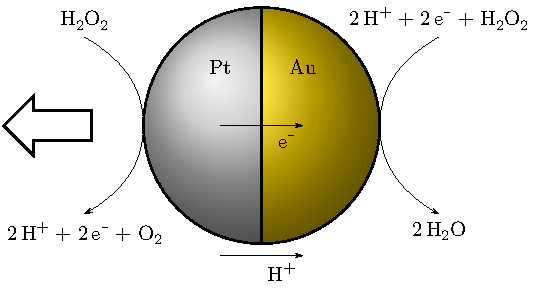
\includegraphics{FIGURES/janus-particle}
  \caption{\label{fig:janus}A Janus swimmer, having a catalytic surface on both hemispheres, may support two different (redox) reactions. This results in breaking of reflection symmetry which propels the particle in the direction of the large arrow.}
\end{figure}

Let us begin by describing the chemical swimmer that we wish to model. Consider a Janus swimmer, see Fig.~\ref{fig:janus}, consisting of \ch{Pt} on one hemisphere and \ch{Au} on the other hemisphere. Both surfaces catalytically induce a forward reaction (there is an abundance of hydrogen peroxide and absence of products), here~\cite{Gibbs_10,Wheat_10}
\begin{align}
  \label{eq:H2O2}
  \ch{
    H2O2 &->[ Pt ] 2 H^+ + 2 e^- + O2 \\
    2 H^+ + 2 e^- + H2O2 &->[ Au ] 2 H2O
  }
\end{align}
The block arrow in the sketch points in the direction of movement induced by the reaction. We refer to upper and lower hemisphere (or half-space) in the following, as two regions that are determined with respect to the orientation of the particle and the plane through the center of the particle, with the orientation as its normal. In the present case one might choose \ch{Au} as the upper hemisphere and \ch{Pt} as the lower hemisphere. The reaction region is bounded by the \textit{reaction range}: $r$.

Examining the reactions in Eq.~\eqref{eq:H2O2}, we observe that catalytic surfaces induce a reactions that produce charged species by consuming hydrogen peroxide. Assuming that it is the change in distribution of charged species that lead to motion of the swimmer, a process refered to as self-electrophoresis~\cite{Gibbs_10,Wheat_10}, then a minimal model for this would be 
\begin{align}
  \label{eq:simple}
  \ch{
    A &->[ C^{+} ] B \\
    B &->[ C^{-} ] A 
  }
\end{align}
where on the upper half of the catalyst $C^{+}$ a species $A$ is converted into $B$, and on the lower half the opposite reaction takes place. Note that when $A$ and $B$ are charged, this reaction conserves charge, provided the rates are equal. 

In \es\, we model this reaction as follows. Inside the reaction range, we react only rectant-product pairs. The particles in a pair are swapped from top to bottom with a rate prescribed by Eq.~\eqref{eq:prob}, and a pair may be swapped only once per MD time step, to avoid a no-net-effect situation. That is, we allow an exchange move only when the following conditions are met:
\begin{enumerate}
\item Both partners of the reactant-product pair have to reside within
  the reaction range.
\item The product has to reside in the upper half-space of the
  reaction range.
\item The reactant has to reside in the lower half-space of the
  reaction range.
\end{enumerate}
The situation is illustrated in Fig.~\ref{fig:nc}.

\begin{figure}
  \centering
  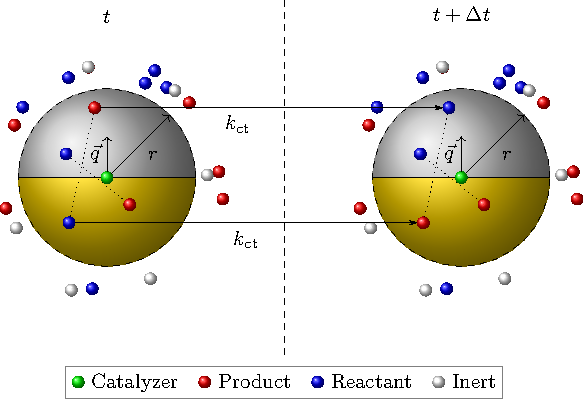
\includegraphics{FIGURES/number-conserving}
  \caption{\label{fig:nc}Illustration of the catalytic scheme. The cut-off range of $r$ around the catalyzer (green) is subdivided into two half-spaces. A reactant-product pair (blue and red connected by dotted line)is converted by swapping them if the pair is selected, and only if the product (red) resides in the upper half-space (silver background) and the corresponding reactant (blue) resides in the lower half-space (gold background). The catalytic reaction leads to a conversion of one reactant-product pair of particles in this example, denoted by the arrows annotated with $k_{\text{ct}}$. The second reactant-product pair within the reaction range is not viable for conversion. Additionally, particles in a pair may only undergo one exhange per time step.}
\end{figure}

\subsection{Usage in \es}

Catalytic reactions can be enabled in \es\ by compiling in the eponymous feature \code{CATALYTIC_REACTIONS} and the \code{ROTATION} feature to provide the particles with an orientation vector. In \es\ the orientation of the particle is defined by a quaternion; this in turn defines a rotation matrix that acts on the particle's initial orientation (along the $z$-axis), which then defines the particles current orientation~\cite{UG,Limbach_06,Arnold_13}.

To setup the reaction there is the \es\ command \codees{Reaction}, which operates on particle types. The general syntax is
\begin{espresso}
reaction reactant_type R catalyzer_type C product_type P range r ct_rate k_ct
    [react_once on/off]
\end{espresso}
The parameter \codees{react_once} is optional and can be left out, the default values is \codees{react_once off}.

To set up a reaction between particles with types 1 and 2, where particles of type 3 act as catalyzers with a reaction range of 1.5 around them and a reaction rate of 20, one inputs
\begin{espresso}
reaction reactant_type 1 catalyzer_type 3 product_type 2 range 1.5 ct_rate 20
\end{espresso}
Here, we have left out the optional parameter \codees{react_once}, however, its meaning is important. Briefly, the parameter determines whether a particle can take part in a only single reaction move per time step. In the case of multiple catalyzers in the system a particle might be tagged for reaction several times by different catalyzers because their reaction ranges overlap and the reactant is inside this overlap. This can be prevented by setting \code{react_once on}. That way the reaction rate is independent of the density of catalyzers. This can be convenient if one wants to model several catalyzer particles that are in close proximity to one another.

\noindent\textbf{Important:} Due to the method of implementation there can only be one reaction. You can alter the reaction parameters, but you may not change the reaction partners. Note also that the reaction move does not really exchange the particles, it only exchanges their type (and their charge, if \es\ was compiled with \code{ELECTROSTATICS}). This means that the particle numbers do not change. To track how frequently a particle undergoes a reaction, one must therefore track the properties of a particle via the particle number.

\section{Configuring \es\ for Catalytic Reactions}

For this tutorial to work you need a version of \es\ containing the catalytic reactions feature. Check out the \es\ online repository at \url{https://github.com/espressomd/espresso}. If you have installed \code{git}, you can issue on the command line
\begin{bash}
$ git clone https://github.com/espressomd/espresso.git
\end{bash}
Now you are ready to build \es. Change to the newly created directory and use the following commands to configure \es\ for compilation.
\begin{bash}
$ mkdir build
$ cd build
$ cmake ..
\end{bash}
After this, you will need to copy the \code{myconfig-sample.hpp} file into \code{myconfig.hpp} and select the appropriate \code{FEATURES} in the latter.
\begin{bash}
$ cp myconfig-sample.hpp myconfig.hpp
\end{bash}
To run all the tutorials you need to uncomment the following \code{FEATURES}:
\begin{lstlisting}[language=c]
#define ROTATION
#define ROTATIONAL_INERTIA
#define LANGEVIN_PER_PARTICLE
#define CATALYTIC_REACTIONS
#define LENNARD_JONES
\end{lstlisting}
Now you are ready to build \es.
\begin{bash}
$ make -j N
\end{bash}
with $N$ the number of processes used to build. Next you can unpack the archive with the tutorial files in this directory. You will find two folders, one called `EXERCISES' and one called `SOLUTIONS'.

\section{The Enhanced-Diffusion Tutorial}

In the folder `EXERCISES' you will find the \code{reaction.tcl} file. It is a tutorial to demonstrate that our approach to catalytic reactions leads to enhanced diffusion of the catalyzer. When you begin, the code is incomplete and will produce errors when evaluated in \es. It needs your input to function properly. A fully functional file exists in the `SOLUTIONS' folder, but we recommend that you try solving the exercises on your own first.

To start the exercises, go into the `EXERCISES' directory and invoke \es\ on the script
\begin{bash}
$ ./../build/Espresso reaction.tcl 0
\end{bash}
where the parameter \code{0} determines whether the reaction is enabled. Here, 0/1 corresponds to reaction off/on. At this stage, executing the above line will cause an error, as the exercise has not yet been completed.

\subsection{Structure of the Simulation}

Let us walk through the script. It is best to open the file while reading this. You should have learned about everything that does not have to with catalytic reactions in previous tutorials. If you find that you are unfamiliar with any concept, while you are going though the script, it might be better to go back and complete the other tutorials first.

First, we read the activity parameter from the command line and verify it. Then we set up some general simulation parameters, such as box length, radius of the colloid, concentration of reactant and products, and the reaction rate. Next, we setup the thermostat parameters, but do not enable it yet. Before we can set up the colloid and the small particles around, the first two exercises have to be completed. The script continues, by setting up interactions between the colloid and the smaller particles and, most importantly, the reaction. The syntax for setting up a reaction is given above in the section ``Usage in \es''.

Warmup is performed by the \codees{minimize_energy} routine. It has several advantages over traditional force-capping warmup, which you will learn about when completing the associated exercise. Next, the thermostat is enabled and the equilibration is performed. Finally, we perform five production runs in which we measure the mean-square displacement (MSD) and the angular velocity auto-correlation function (AVACF).

\subsection{What to Expect}

Once you have completed all the tasks in the exercise script, the time has come to run the actual simulation. Run the script twice, once with the activity parameter set to 0 and once set to 1. You will have two directories: \code{active-system} and \code{passive-system}. These contain MSD and AVACF data files numbered consecutively over the different runs.

It is now your job to average over these five files. You can do this in \code{gnuplot} or the scripting language of your choice. The MSD files have five columns each. The first two columns are time and samples, the last three are $x$, $y$, and $z$. The AVACF files have only three columns, where the first two are also time and samples and the third is the AVACF averaged over all spatial components. For the MSD we still have to average over the three spatial dimensions.

\begin{figure}[tb]
  \centering
  \leavevmode\hfill
  \begin{minipage}[t]{.45\linewidth}
    \centering
    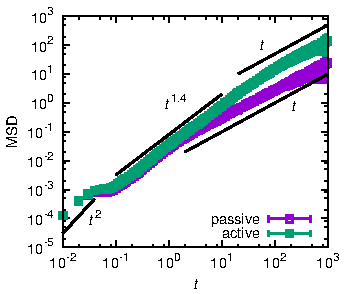
\includegraphics{FIGURES/msd}
    \caption{Averaged MSD over five runs with standard error on the
      error bars for both, the active and the passive system. The
      black lines serve as a guide to the eye and indicate the
      dependence of the MSD on the time $t$.}
    \label{fig:msd}
  \end{minipage}
  \hfill
  \begin{minipage}[t]{.45\linewidth}
    \centering
    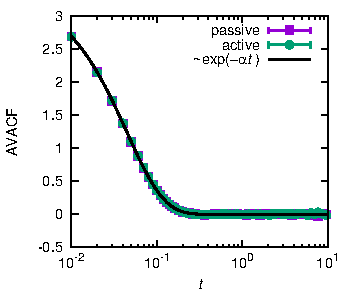
\includegraphics{FIGURES/avacf}
    \caption{The AVACF for the same system as in
      figure~\ref{fig:msd}. Note that the activity does not influence
      the rotational behavior.}
    \label{fig:avacf}
  \end{minipage}
  \hfill\null
\end{figure}

When we have extracted the mean (and recommendably the standard error) we can plot it over time to achieve plots similar to the ones shown in Figs.~\ref{fig:msd} and~\ref{fig:avacf}. It is clear that the reaction facilitates enhanced translational diffusion, while leaving the rotational diffusion unaffected. We refer to the Active Matter tutorial for a lengthier discussion of the concept of enhanced diffusion.

Note that a passive particle shows a $t^{2}$ ballistic regime, typical for Langevin type simulations, followed by an intermediate regime, where the slope changes gradually to the long-time diffusive $t$. The active swimmer, shows similar behavior. However, the intermediate regime is stretched, with the long-time diffusion setting in only at around $t = 10$  --- this corresponds to one rotational diffusion time. The rotational diffusion remains unaffected by the particle catalyzing solutes in its surrounding.

\section{Concluding Remarks}

With that, you have come to the end of this tutorial. We hope you found it informative and that you have a sufficient understanding of the way to deal with catalytic reactions in \es\ to set up simulations on your own.

\section*{References}

\bibliographystyle{unsrt}
\bibliography{refs}

\end{document}

%%% Local Variables: 
%%% mode: latex
%%% End:
